\section{Home}

Die Startseite des ACPs gibt eine allgemeine Schnellerklärung über alle Seiten des ACPs und ist die erste Seite auf der man nach der Anmeldung landet. Neben den allgemeinen Erklärungen stehen auf der Startseite Statistiken und Systeminformationen wie CPU-Auslastung, Laufzeit des Servers, RAM-Nutzung usw.

\begin{figure}[ht]
    \centering
    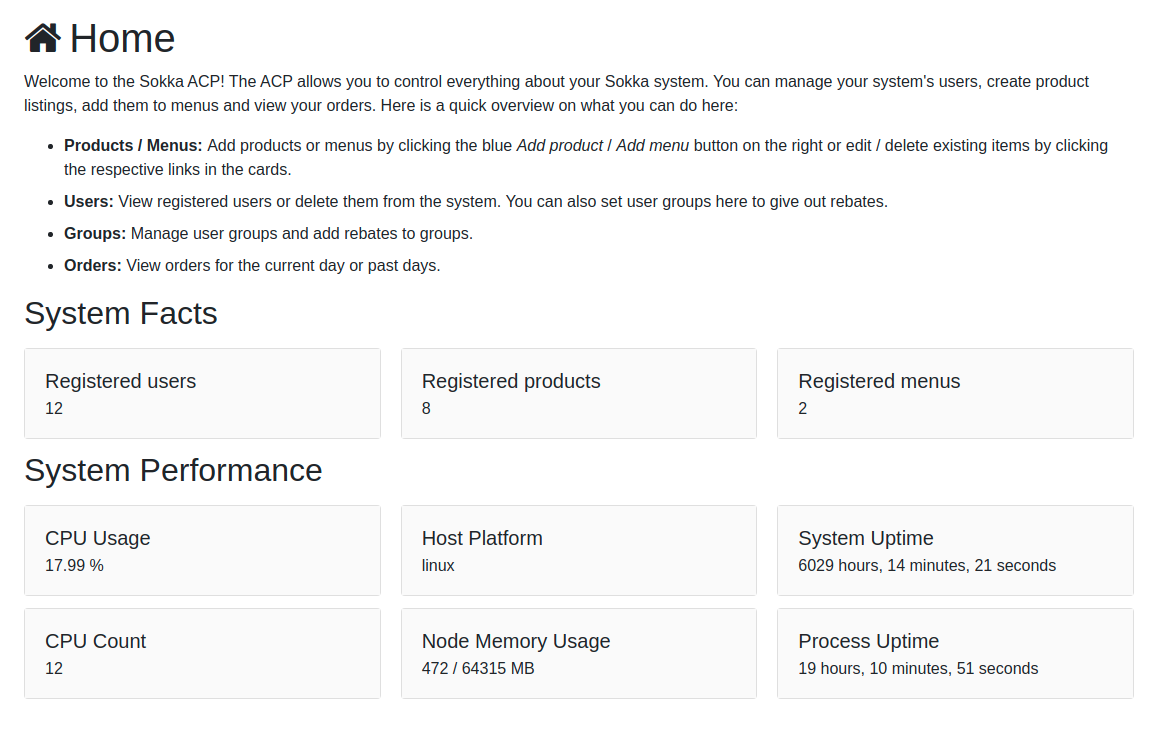
\includegraphics[width=0.8\textwidth]{images/ACP/home.png}
    \caption{Die Startseite des Sokka-ACPs}
\end{figure}

Die Informationen unter \textbf{System Facts} und \textbf{System Performance} aktualisieren sich alle fünf Sekunden automatisch. Für das Auslesen der Performance-Daten wird die Library \lstinline{os-utils} verwendet.
